\begin{figure}[t]
    \centering
    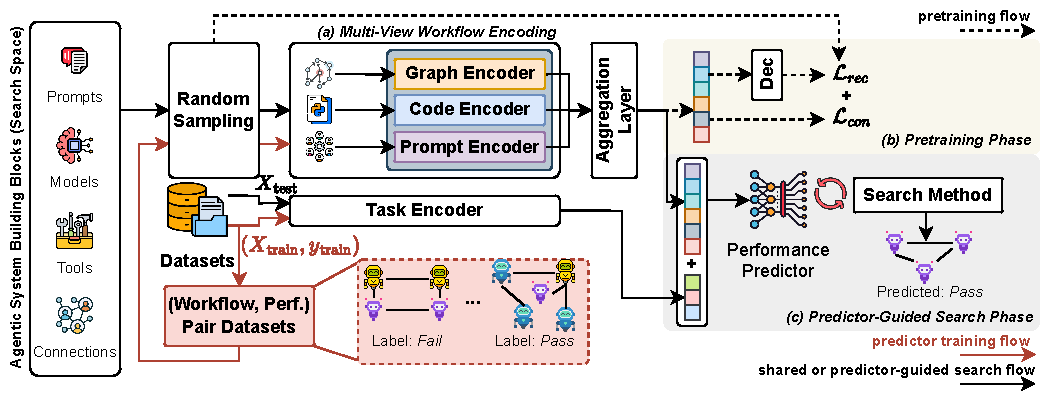
\includegraphics[width=\textwidth]{figures/framework_overview.pdf}
    \vspace*{-0.6cm}
    \caption{Overview of our \ours{} framework. A \textbf{(a) multi-view workflow encoder} is designed to encode a set of agentic workflows from graph, code, and prompt aspects into unified representations, which serve as features for training the predictor. In the \textbf{(b) pretraining phase}, the encoder learns these representations on unlabeled workflows spanning diverse tasks and domains, using cross-domain unsupervised pretraining objectives. In the \textbf{(c) predictor-guided search phase}, a performance predictor is trained on a small (workflow configuration, performance) dataset to classify configurations as pass or fail, and subsequently guides the search toward promising configurations.} \label{figure:overall_framework}
    \vspace*{-0.3cm}
\end{figure}


\vspace*{-0.1cm}
\section{Methodology: Agentic Predictor} \label{section:method}

\vspace*{-0.2cm}
\subsection{Problem Formulation}
\vspace*{-0.2cm}

Let an agentic workflow be denoted as $\mathcal{W} = \{\mathcal{V}, \mathcal{E}, \mathcal{P}, \mathcal{C}\}$, where $\mathcal{V} = \{v_i\}_{i=1}^{N}$ represents the set of $N$ agents, $\mathcal{E}$ denotes the set of edges defining the connections between agents, and $\mathcal{P} = \{p_i\}_{i=1}^{N}$ denotes the system prompts for each agent $i$. $\mathcal{C}$ represents the complete code specifying the logic and structure of the workflow. Thus, the workflow $\mathcal{W}$ is represented as a directed acyclic graph\,(DAG).

Given a task description $T$, the workflow $\mathcal{W}$ autonomously executes agents in topological order, where the $i$-th agent receives the task description $T$ along with the outputs $y$ from its predecessor agents. Formally, the input to agent $i$ is defined as $\mathcal{X}_{i} = \{T\} \cup \{y_j : v_j \in \mathcal{N}_i^{\text{(in)}}\}$, where $\mathcal{N}_i^{\text{(in)}}$ denotes the set of predecessor agents of agent $i$, and $y_j$ is the output of agent $j$. The output $y_i$ of agent $i$ is generated by querying an LLM: $y_i = \mathrm{LLM}(\mathcal{X}_i, p_i)$. After executing all agents, the final response of the agentic workflow is defined as $r = f_{\mathrm{LLM}}(\mathcal{W}, T)$, where $f_{\mathrm{LLM}}$ represents the overall execution process of the given LLM. Generally, this process is repeated for the evaluation of $r$, which incurs significant computational and financial overhead.

In contrast, this paper aims to design a predictive model $\mathcal{M}$ that efficiently estimates the final performance of an agentic workflow $\mathcal{W}$ on a given task description $T$, without requiring costly LLM invocations. Therefore, we treat the workflow $\mathcal{W}$ and task description $T$ as inputs to the predictor $\mathcal{M}$, which outputs the estimated performance $\hat{e}$. Formally, $\hat{e} = \mathcal{M}_{\Theta}(\mathcal{W}, T)$, where $\Theta$ denotes the learnable parameters of the performance predictor.

\textbf{Learning Objective}. Given the workflow $\mathcal{W}$, task description (or query) $T$, and performance predictor $\mathcal{M}_{\Theta}$ parameterized by $\Theta$, we aim to find the optimal $\Theta$ that minimizes the error between the estimated performance $\hat{e}$ and the ground-truth performance $e$. Formally, we solve
\begin{equation} \label{eq:learning_objective}
    \underset{\Theta}{\mathrm{min}}~\mathbb{E}_{(\mathcal{W}, T)} [\mathcal{L}(e, \hat{e})],
\end{equation}
where $\mathcal{L}(\cdot,\cdot)$ is a loss function that quantifies the discrepancy between the ground truth and the predicted performance. $\mathcal{L}$ can be either the cross-entropy loss or the mean squared error loss, depending on whether the prediction task is formulated as a classification or regression problem.


\subsection{Framework Overview}
We present an overview of our \ours{} framework in \autoref{figure:overall_framework}. First, the multi-view workflow encoder integrates key aspects of an agentic workflow---graph structures $(\mathcal{V}, \mathcal{E})$, code implementations $\mathcal{C}$, and system prompts $\mathcal{P}$---into a unified representation $\mathcal{F}$. Integration is achieved via modality-specific encoders followed by an aggregation layer that consolidates features across modalities. Second, when labeled instances are scarce, we refine these representations with unsupervised objectives, reconstruction and contrastive learning, to improve generalization and adaptability across diverse tasks and configurations. Third, a dedicated performance predictor $\mathcal{M}_{\Theta}$ is trained on a labeled set (often small) comprising workflow configurations $\mathcal{W}$, task descriptions $T$, and observed performance outcomes $e$. Finally, with the trained predictor, we perform a predictor-guided search that efficiently ranks and selects promising workflow configurations without incurring expensive LLM calls. Because \ours{} is search-agnostic, we deliberately do not commit to a specific search algorithm within the framework.

\subsection{Multi-View Workflow Encoding} \label{section:multiview_encoding}
Motivated by recent findings in the NAS literature\,\citep{EncodingNAS_NeurIPS_20, FLAN_ICML_24, PASTA_TETCI_24}, which show that architecture representations strongly influence predictor performance, we argue for expressive, comprehensive representations tailored to agentic workflows. Because agentic workflows differ fundamentally from traditional neural architectures, conventional graph-based encodings alone are insufficient. Although DAGs naturally capture explicit inter-agent communication and dependencies, they omit crucial implicit signals such as tool-usage patterns, code structure, computational complexity, and the nuanced semantics present in agent prompts. To address these limitations, we propose a multi-view encoding scheme that integrates complementary representations at multiple granularities, with each view capturing distinct yet essential aspects of LLM-based agentic workflows.
\begin{itemize}[leftmargin=10pt, nosep, noitemsep]
    \item \textbf{Graph View} explicitly models structural dependencies and direct interactions among agents, emphasizing inter-agent communication channels. We denote the graph view as $\mathcal{G} = (\mathcal{V}, \mathcal{E})$.
    \item \textbf{Code View} implicitly encodes program-level semantics, control and logical sequence, computational complexity, and patterns of tool usage inherent in workflow implementations $\mathcal{C}$.
    \item \textbf{Prompt View} provides semantic embeddings that capture agent roles, behavioral specifications, and broader contextual guidance embedded within system and instruction prompts $\mathcal{P}$.
\end{itemize}
Our rationale for adopting this multi-view framework is that aggregating heterogeneous information sources reduces representation bias, thereby improving both robustness and predictive accuracy.


\subsubsection{Encoder Networks}
We now detail the components of our proposed multi-view workflow encoding method for performance prediction in agentic workflows using neural networks. Let $\mathrm{Enc}(\cdot)$ denote an encoder function that maps a candidate workflow---composed of $(\mathcal{G}, \mathcal{C}, \mathcal{P})$---into $d$-dimensional Euclidean space, i.e., $\mathrm{Enc}(\cdot) : (\mathcal{G}, \mathcal{C}, \mathcal{P}) \to \mathbb{R}^d$. Given the heterogeneous nature of workflow configurations, we design three specialized encoder networks, each responsible for learning a representation corresponding to a distinct view. These view-specific representations are then aggregated into a shared latent space, denoted by $\mathbf{Z} = \mathrm{Enc}(\mathcal{G}, \mathcal{C}, \mathcal{P})$, where $\mathbf{Z} \in \mathbb{R}^d$. This continuous latent representation is used to train the performance predictor $\mathcal{M}_{\Theta}$ (see \S\ref{section:predictor_search}). The individual encoders for each view are integrated into a unified architecture as described below.

\textbf{Graph Encoder}. We employ graph neural network\,(GNN) layers to encode graph-based representations. The workflow is modeled as a DAG in which each edge encodes a unidirectional message channel. Rather than relying on a single graph, we adopt a \emph{multi-graph} approach that integrates node features from multiple views, including agent-specific definitions and function-call implementations at each agent node. We instantiate this multi-graph representation with three graph views constructed from a workflow $\mathcal{W}$. In the \emph{prompt graph} $\mathcal{G}_{\text{prompt}}$, node features are obtained by pooling the embeddings of each agent's system and instruction prompts. In the \emph{code graph} $\mathcal{G}_{\text{code}}$, node features correspond to the function-call code associated with each agent. In the \emph{operator graph} $\mathcal{G}_{\text{operator}}$, node features encode operator types and their definitions. All three graphs share the same node and edge set, where edges can be derived from an abstract syntax tree as suggested by \citet{FLORA_Bench_25}. 

We then obtain view-specific node embeddings $\mathbf{H}_{\text{prompt}}=\mathrm{GNN}(\mathcal{G}_{\text{prompt}})$, $\mathbf{H}_{\text{code}}=\mathrm{GNN}(\mathcal{G}_{\text{code}})$, and $\mathbf{H}_{\text{operator}}=\mathrm{GNN}(\mathcal{G}_{\text{operator}})$ in $\mathbb{R}^{N\times d}$, stack them along a view dimension to form $\mathbf{X}\in\mathbb{R}^{N\times V\times d}$ with $V = 3$, and apply a cross-view self-attention block with residual connection and layer normalization $\hat{\mathbf{X}} = \mathrm{LN}\!\left(\mathrm{MHA}(\mathbf{X},\mathbf{X},\mathbf{X}) + \mathbf{X}\right)$, where $\mathrm{MHA}$ is multi-head attention applied across views for each node (the sequence axis is the view axis; topology is unchanged). 

Next, a view-attention pooling module computes per-node attention weights with a $L$-layer multi-layer perceptron\,(MLP) and $\tanh$ nonlinearity, followed by a softmax over views, and produces a weighted sum across views $\mathbf{H} = \mathrm{ViewAttnPool}(\hat{\mathbf{X}})\in\mathbb{R}^{N\times d}$. Finally, a graph readout $G_{\mathrm{pool}}$ aggregates node embeddings into a single graph representation, $\mathbf{Z}_{\mathcal{G}} = G_{\mathrm{pool}}\!\left(\mathbf{H}\right) = G_{\mathrm{pool}}\!(\mathrm{ViewAttnPool}(\mathrm{CrossGraphAttn}(\mathbf{X})))$, which preserves edge directionality from the upstream GNN while capturing cross-view contextual dependencies at the node level before graph-level summarization. Here, $\mathrm{CrossGraphAttn}$ enriches each node with multi-view contextual dependencies, while $\mathrm{ViewAttnPool}$ highlights which views are most informative.

\textbf{Code Encoder}. While $\mathcal{G}_{\text{code}}$ and $\mathcal{G}_{\text{operator}}$ primarily encode structural information derived from the different workflow graphs, this code encoder is designed to provide a complementary, holistic representation of the entire workflow code. To model the workflow-level embeddings, we use an $L$-layer MLP to extract latent semantic features, enabling the model to learn intricate computational logic and tool interactions at a \emph{global} level. The code representation is computed as $\mathbf{Z}_{\mathcal{C}} = \mathrm{MLP}_\mathcal{C}(\mathcal{C})$.

\textbf{Prompt Encoder}. Instead of encoding agent prompts solely as node-level features\,\citep{FLORA_Bench_25}, we use a separate $L$-layer MLP to encode the \emph{entire} workflow instruction prompt holistically. This approach captures role descriptions, behavioral intents, and global context---resulting in richer and more semantically informed representations. The prompt encoding is $\mathbf{Z}_{\mathcal{P}} = \mathrm{MLP}_{\mathcal{P}}(\mathcal{P})$.

\textbf{Aggregation Layer}. The representations from the graph, code, and prompt encoders---$\mathbf{Z}_{\mathcal{G}}$, $\mathbf{Z}_{\mathcal{C}}$, and $\mathbf{Z}_{\mathcal{P}}$---are concatenated and passed through a final MLP layer. This aggregation mechanism adaptively integrates information across all views, enabling the model to emphasize the most contextually relevant aspects. The final output of the encoder $\mathrm{Enc}(\cdot)$ is computed as $\mathbf{Z} = \mathrm{MLP}([\mathbf{Z}_{\mathcal{G}}, \mathbf{Z}_{\mathcal{C}}, \mathbf{Z}_{\mathcal{P}}])$.

Consequently, the aggregation layer acts as a \emph{learnable} fusion module. The attention-based graph encoder produces $\mathbf{Z}_{\mathcal{G}}$ with cross-view interactions already embedded, and the downstream fusion assigns task-dependent importance to the graph-, code-, and prompt-level representations, rather than treating all views as equally informative. These encoders learn not only from different workflow perspectives but also at varying levels of granularity, specifically, at the graph level for agent interactions, the code level for logical structures, and the prompt level for agent-specific instructions. 

\subsubsection{Decoder Networks} 
The decoder is a generative module that reconstructs $\hat{\mathcal{G}}$, $\hat{\mathcal{C}}$, and $\hat{\mathcal{P}}$ from the latent variables $\mathbf{Z}$ to encourage learning generalizable representations of agentic workflows. It consists of a stack of MLP layers. For simplicity, the decoder outputs the modality-specific \emph{input embedding} vectors of $\mathcal{G}$, $\mathcal{C}$, and $\mathcal{P}$. Accordingly, we parameterize $\mathrm{Dec}(\cdot)$ with an MLP and define $\hat{\mathcal{G}}=\mathrm{MLP}(\mathbf{Z}_{\mathcal{G}})$, $\hat{\mathcal{C}}=\mathrm{MLP}(\mathbf{Z}_{\mathcal{C}})$, and $\hat{\mathcal{P}}=\mathrm{MLP}(\mathbf{Z}_{\mathcal{P}})$. This decoder is used only during pretraining for self-supervised reconstruction of modality-specific embeddings from $\mathbf{Z}$ and is not part of the encoding path at inference time.



\subsection{Cross-Domain Unsupervised Pretraining} \label{section:pretraining}
In real-world scenarios, labeled performance data for agentic workflows are scarce due to costly evaluation. To enable data-efficient training without label leakage, we \emph{optionally} adopt a two-phase strategy. Rather than directly supervising the encoder with performance labels, we first perform cross-domain unsupervised pretraining to obtain rich and generalizable workflow representations $\mathbf{Z}$. No performance labels\,(e.g., success/failure) are used in this stage. The resulting representations improve sample efficiency for downstream prediction, in line with observations in NAS\,\citep{EncodingNAS_NeurIPS_20, arch2vec_NeurIPS_20, CATE_ICML_21, FLAN_ICML_24, PASTA_TETCI_24}. When sufficiently many labels are available, direct supervised learning of the predictor remains feasible.



\textbf{Multi-Task Pretraining}. We train the multi-view encoder on $M$ unlabeled workflow configurations by minimizing a combined loss comprising reconstruction and contrastive objectives: $\mathcal{L}_{rec} = \frac{1}{M} \sum_{i=1}^M \Vert\mathcal{G}_i-\hat{\mathcal{G}}_i\Vert^2 + \Vert\mathcal{C}_i-\hat{\mathcal{C}}_i\Vert^2 + \Vert\mathcal{P}_i-\hat{\mathcal{P}}_i\Vert^2$ and $\mathcal{L}_{con} = \frac{1}{M} \sum_{i=1}^M -\mathrm{log}\frac{\mathrm{exp}(\mathrm{sim}(\mathbf{Z}_i, \mathbf{Z}_j^+)/\tau)}{\sum_{k=1}^M \mathrm{exp}(\mathrm{sim}(\mathbf{Z}_i, \mathbf{Z}_k)/\tau)}$. Here, $\mathcal{G}_i, \mathcal{C}_i, \mathcal{P}_i$ denote the input graph, code, and prompt embeddings, respectively, while $\hat{\cdot}$ denotes reconstructions via modality-specific decoders. Notably, the graph branch reconstructs its own embedding target with a stop-gradient, whereas code and prompt/text are reconstructed in input space. The contrastive loss is instantiated \emph{cross-modally} with in-batch sampling. For each configuration $i$, positives $(\mathbf{Z}_i,\mathbf{Z}_j^+)$ are the index-aligned embeddings of the configuration across two different views (e.g., $\mathcal{G}_i$ with $\mathcal{C}_i$), while negatives are all other configurations within the batch. We symmetrize the objective by swapping anchor/target and average it over the three view pairs $(\mathcal{G},\mathcal{C})$, $(\mathcal{G},\mathcal{P})$, and $(\mathcal{C},\mathcal{P})$. This learning objective encourages the encoder to capture structure- and content-aware signals without observing performance outcomes. Thus, the total loss function is $\mathcal{L}_{enc} = \mathcal{L}_{rec} + \mathcal{L}_{con}$.



\subsection{Performance Predictor} \label{section:predictor_search}
Following the unsupervised pretraining of the multi-view encoder, we introduce a lightweight performance predictor to guide exploration of the large agentic workflow space. This phase enables efficient identification of high-performing configurations with minimal supervision, using only a small set of labeled workflow–performance pairs. As shown in \autoref{figure:overall_framework}(c), our predictor operates on learned workflow embeddings, enriched with task-specific context, to form a joint representation $\mathcal{F}$ used for performance prediction and downstream search.

\textbf{Task Encoder}. To capture task-specific characteristics, we incorporate a Task Encoder that generates high-level semantic embeddings from natural-language task descriptions. These embeddings, derived from pretrained language models\,(e.g., T5 or BERT), provide global context that helps differentiate tasks with similar surface form but distinct functional requirements. The task embedding is concatenated with the multi-view workflow representation, forming $\mathcal{F} = [\mathbf{Z}, \mathbf{T}]$, where $\mathbf{Z}$ is the encoded workflow and $\mathbf{T}$ is the task embedding. For workflow content itself (prompts and code), we pair this with lightweight, domain-specific encoders within the multi-view backbone to balance representational capacity with efficiency. This separation of modalities followed by fusion captures complementary compositional and contextual signals and supports generalization across heterogeneous tasks with varying operational goals and constraints.

The performance predictor is a lightweight prediction head $\mathcal{M}_{\Theta}$\,(e.g., an MLP) trained on a limited set of labeled data ${(X_{\text{train}}, y_{\text{train}})}$, where each $X_{\text{train}}$ corresponds to $\mathcal{F}$ and $y_{\text{train}}$ is the performance label\,(e.g., binary success/failure or a scalar score). We instantiate the objective to match the label type. For binary labels, we use a binary cross-entropy loss, i.e., $\mathcal{L}_{\text{pred}} = - \frac{1}{N} \sum_{i=1}^{N} \left[ e_i \log \hat{e}_i + (1 - e_i) \log (1 - \hat{e}_i) \right]$, where $\hat{e}_i$ is the predicted success probability. For numeric labels, we can use mean squared error, i.e., $\mathcal{L}_{\text{pred}} = \frac{1}{N}\sum_{i=1}^{N} (s_i - \hat{s}_i)^2$. By operating on semantically rich pretrained embeddings, the predictor attains strong accuracy in the low-data regime, enabling label-efficient search.



\textbf{Integration with Workflow Optimization}. With the trained predictor in place, we can perform predictor-guided search to efficiently explore the workflow configuration space. Rather than evaluating each configuration via full execution, we embed candidates into their joint representations $\mathcal{F}$ and score them using the predictor. The top-scoring candidates are selected for evaluation. This substantially reduces computational cost by focusing on the most promising regions of the search space. A simple yet effective instantiation of this strategy uses random search to sample $K$ workflow candidates from the full configuration space, and then ranks them using the learned predictor. We select the top-$k$ configurations, averaged across samples in the benchmark, for evaluation. This predictor-as-ranker setup transforms random search into a label-efficient guided procedure without requiring complex heuristics. Since our main contribution is the performance predictor rather than the optimization algorithm, we focus evaluation on prediction accuracy and ranking quality\,(i.e., workflow utility) in the following section. Additional results on workflow optimization appear in \S\ref{section:workflow_results}.